\documentclass[12pt, oneside]{article}
\usepackage{soto-quiz}
\usepackage{tikz}
\usepackage{fancyhdr}

\newif\ifsolution
\input{solution}

\begin{document}

\lhead{ENSP 202}
\chead{Exercises 6}
\rhead{\today}
%\rhead{Wednesday 26 Mar 2014}
\lfoot{}
\cfoot{}
\rfoot{}
\pagestyle{fancy}

\namebox

\problem{Graphing slopes}

We measure the depth of a tub of dimensions 1 meter by 0.5 meters.
Sketch the flow rate of the faucet into the tub in the second graph.

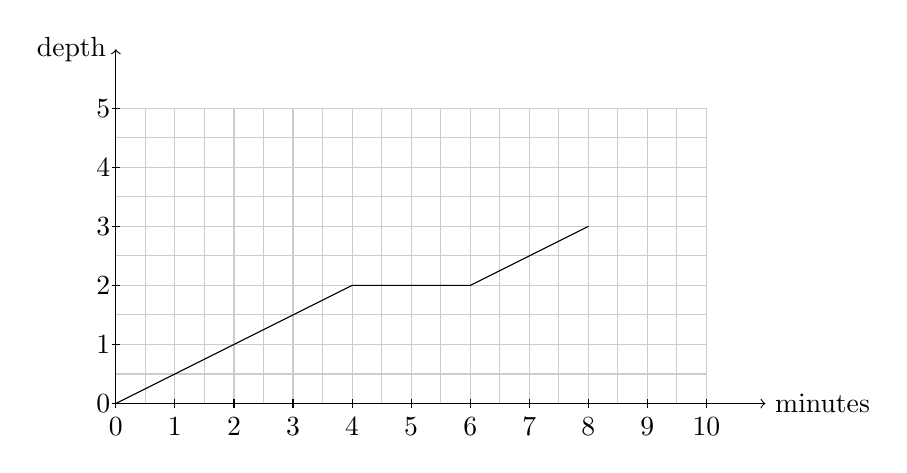
\begin{tikzpicture}[scale=0.75]
\def\sx{1}
\def\sy{1}

% tikz problem with grid to figure out slopes of graph
% Draw thin grid lines with color 40% gray + 60% white
\draw [step=0.5,thin,gray!40] (0, 0) grid (10, 5/\sy);

% Draw x and y axis lines
\draw [->] (0, 0) -- (11.0, 0) node [right] {minutes};
\draw [->] (0, 0) -- (0, 6/\sy) node [left] {depth};

% voltage labels
\foreach \x in {0,1,2,3,4,5,6,7,8,9,10} {
    \draw (\x/\sx, 2pt) -- (\x/\sx,-2pt) node[below] {$\x$};
}

\foreach \y in {0,1,2,3,4,5} {
    \draw (-2pt,\y/\sy) -- (2pt,\y/\sy) node[left] {$\y$};
}



\draw (0,0) -- (4,2) -- (6, 2) -- (8, 3);

\end{tikzpicture}



\solution{
We want to find the rate at which water is being poured into the tub in
volume per minute.  We need to convert our depth into the volume of
water.  To do this we use the estimation that the volume is the length
times the width of the tub times the depth of the water.

We use the depth to find the volume.  Over the first four minutes, the
depth increases from 0 to 2 meters.
The volume then is
$$ V = l \cdot w \cdot depth$$
$$ V = 1m \cdot 0.5m \cdot 2m = 1.0 m^3 $$

The rate is then

$$ \frac{1.0 m^3}{4 min}= 0.25 m^3/min $$

Over the period of time from 4 to 6 minutes, the depth does not increase
so the flow must be zero.  From 6 to 8 minutes the slope is the same.
In a graph, the flow looks like:

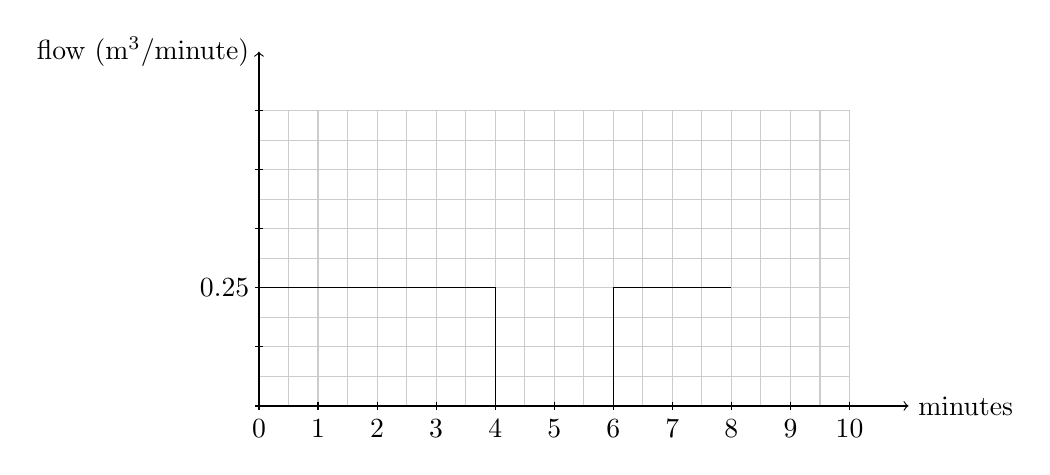
\begin{tikzpicture}[scale=0.75]
\def\sx{1}
\def\sy{1}

% tikz problem with grid to figure out slopes of graph
% Draw thin grid lines with color 40% gray + 60% white
\draw [step=0.5,thin,gray!40] (0, 0) grid (10, 5/\sy);

% Draw x and y axis lines
\draw [->] (0, 0) -- (11.0, 0) node [right] {minutes};
\draw [->] (0, 0) -- (0, 6/\sy) node [left] {flow (m$^3$/minute)};

% voltage labels
\foreach \x in {0,1,2,3,4,5,6,7,8,9,10} {
    \draw (\x/\sx, 2pt) -- (\x/\sx,-2pt) node[below] {$\x$};
}

\foreach \y in {0,1,2,3,4,5} {
    \draw (-2pt,\y/\sy) -- (2pt,\y/\sy) node[left] {};
}

\draw (0,2) node[left] {0.25};

\draw (0, 0) -- (0,2) -- (4,2) -- (4,0) -- (6,0) -- (6,2) -- (8,2) ;


\end{tikzpicture}

}


\problem{Mass of Carbon}

The effective volume of the atmosphere is about 4.2 billion cubic
kilometers.  If the density of carbon dioxide is 1.9 kg/cubic meter and
the amount of carbon in the atmosphere is 397 ppm, what is the total
mass of carbon?  (Note that the actual volume of the atmosphere is different
than the effective volume.  The effective volume allows us to make
calculations more easily.)

\solution{
To convert, we use 1000 meters equals 1 km and remember that this is a
cubic measure
$$ 4.2 \cdot 10^9 km^3 \cdot \frac{(1000m)^3}{(1km)^3} = 4.2 \cdot
10^{18} m^3$$

For every unit volume of atmosphere, if we divide it into 1 million
equal volumes, with only one gas in each, 397 of those tiny volumes will
be carbon dioxide.
$$ \ufrac{397}{parts carbon dioxide}{1}{million parts atmosphere} $$

We multiply the total mass of the atmosphere by the fraction of carbon
dioxide by the density of carbon dioxide.
$$ 4.2 \cdot 10^{18} cubic meters
\ufrac{397}{parts carbon dioxide}{1}{million parts atmosphere}
\ufrac{1.9}{kg}{1}{cubic meter} = 3168 \cdot 10^{12} kg$$
}




\end{document}

